\documentclass{sig-alternate}

\usepackage{url}
\usepackage{amsmath}
\usepackage{graphicx}
\usepackage{subfigure}
\usepackage{threeparttable}
\usepackage{pdflscape}
\usepackage{array}
\usepackage{color}

\begin{document}

\title{The Bug Catalog of the Maven Ecosystem}

\numberofauthors{1}

%\author{
%% 1st. author
%\alignauthor
%Dimitris Mitropoulos\\
%       \affaddr{Athens University of Economics and Business}\\
%       \affaddr{Department of Management Science and Technology}\\
%       \email{dimitro@aueb.gr}
%% 2nd. author
%\alignauthor Vassilios Karakoidas\\
%       \affaddr{Athens University of Economics and Business}\\
%       \affaddr{Department of Management Science and Technology}\\
%       \email{bkarak@aueb.gr}
%% 3rd. author
%\alignauthor Panos Louridas\\
%       \affaddr{Athens University of Economics and Business}\\
%       \affaddr{Department of Management Science and Technology}\\
%       \email{louridas@aueb.gr}
%\and  % use '\and' if you need 'another row' of author names
%% 4th. author
%\alignauthor Georgios Gousios\\
%       \affaddr{Delft University of Technology}\\
%       \affaddr{Software Engineering Research Group}\\
%       \email{G.Gousios@tudelft.nl}
%% 5th. author
%\alignauthor Diomidis Spinellis\\
%       \affaddr{Athens University of Economics and Business}\\
%       \affaddr{Department of Management Science and Technology}\\
%       \email{dds@aueb.gr}
%}

\def\aueb{\textsuperscript{*}}
\def\tud{\textsuperscript{\dag}}

\author{
  Dimitris Mitropoulos\aueb \and Vassilios Karakoidas\aueb \and Panos Louridas\aueb \and Georgios Gousios\tud \and Diomidis Spinellis\aueb \\
  \begin{tabular}{ccc}
  \affaddr{\aueb Department of Management Science and Technology} & & \affaddr{\tud Software Engineering Research Group}\\
    \affaddr{\aueb Athens University of Economics and Business} & & \affaddr{\tud Delft University of Technology}\\
   \affaddr{Athens, Greece} & & \affaddr{Delft, the Netherlands}\\
   \email{\{dimitro,bkarak,louridas,dds\}@aueb.gr}& & \email{g.gousios@tudelft.nl} \\
  \end{tabular}
}

\maketitle
\begin{abstract}
Examining software ecosystems can provide the research community
with useful information. To examine the ecosystem of
the Maven Central Repository (approximately 265{\sc gb} of data),
we performed an experiment where we statically analyzed the
repository to detect its software bugs. For our analysis we
used FindBugs, a tool that examines Java bytecode to detect
numerous types of bugs. In this paper we present our data collection
experiment and show our findings regarding software evolution.
\end{abstract}

\category{D.2.4}{Software Engineering}{Software/Program Verification}[Statistical methods]
\category{D.2.5}{Software Engineering}{Testing and Debugging}[Code inspections and walk-throughs]
\category{D.2.7}{Software Engineering}{Distribution, Maintenance, and Enhancement}[Version control]

\terms{Static Analysis, Software Ecosystems}

\keywords{Maven Repository, FindBugs, Software Bugs}

\section{Introduction}
\label{sec:intro}

A software ecosystem can be seen as a collection of software projects,
which are developed and co-evolve in the same environment~\cite{LL10}.
Components can be interdependent and have multiple versions.
Examples of such ecosystems include Python's
{\sc p}y{\sc py}\footnote{\url{http://pypy.org/}}
(Python Package Index), Perl's
{\sc cpan}\footnote{\url{http://www.cpan.org/}}
(Comprehensive Perl Archive Network), Ruby's
RubyGems\footnote{\url{http://rubygems.org/}}
and the Maven Central Repository.\footnote{\url{http://mvnrepository.com/}}

Maven is a build automation tool used primarily for Java projects and it is
hosted by the Apache Software Foundation.\footnote{\url{http://maven.apache.org/}}
It uses {\sc xml} to describe the software project being built, its dependencies
on other external modules, the build order, and required plug-ins.
To build a software component, it dynamically downloads Java libraries
and Maven plug-ins from the Maven central repository,
and stores them in a local cache. The repository can be updated with
new projects and also with new versions of existing projects
that can depend on other versions.

To statically analyze the Maven repository
we used {\it FindBugs},\footnote{\url{http://findbugs.sourceforge.net/}}
a static analysis tool that examines bytecode to detect software bugs
and has already been used in research~\cite{AP10,SHP06}.
Specifically, we ran FindBugs on all the project versions of all
the projects that exist in the repository
to identify all bugs contained in it.

In this paper we present: a) the experiment performed to obtain the
collection of the metric results that the FindBugs tool produces 
for every project version of the repository (115,214 {\sc jar}s)
and b) how researchers can use the dataset and include it in their research.

\begin{table}
\centering
\begin{tabular}{l r}
\hline
Measurement & Value\\
 \hline
Projects & 17,505\\
Versions (total) & 115,214\\
Min (versions per project) & 1\\
Max (versions per project) & 338\\
Mean (versions per project) & 6.58\\
Median (versions per project) & 3\\
Range (over versions) & 337\\
1$^{st}$ Quartile (over versions) & 1\\
3$^{rd}$ Quartile (over versions) & 8\\
\hline
\end{tabular}
\caption{Descriptive statistic measurements for the Maven repository.}
\label{tbl:repository}
\end{table}

\section{Data Collection Experiment}
\label{sec:exp}

First, we scanned the Maven repository only
for appropriate {\sc jar}s and created a list that included them.
This is because FindBugs analyzes applications written in Java,
and the Maven repository hosts projects from
languages other than Java such as Scala, Groovy,
Clojure, etc. Thus we filtered out such projects.
In particular, we obtained a snapshot (January 2012) of
the repository and handled it locally to retrieve a list of all
the names of the project versions that existed in it.
The statistic measurements concerning the repository can be seen in 
Table~\ref{tbl:repository}.

With the {\sc jar} list at hand, we created a series of processing tasks
and added them to a task queue mechanism (a Rabbit{\sc mq} message
broker). Then we executed twenty five workers (custom Python scripts)
that checked out tasks from the queue, processed each project version
and stored the results to the data
repository (a Mongo{\sc db} database system).

A typical processing cycle of a worker included the following steps: after
the worker spawned, it requested a task from the queue. This task contained
the {\sc jar} name, which was typically a project version that was downloaded locally.
First, specific {\sc jar} metadata were calculated and stored. Such metadata included
its size, its dependencies, and a number that represented the chronological order of the
release. This order was derived from an {\sc xml} file that
accompanies every project in the Maven repository called {\it
maven-metadata.xml}. Then, FindBugs was invoked by the worker and its results were
also stored in the data repository. 
FindBugs separates software bugs into nine
categories\footnote{\url{http://findbugs.sourceforge.net/bugDescriptions.html}}
(including Bad Practice, Security, Performance and others)
and reports bug collections that include all the bugs discovered in a
{\sc jar} file. For every registered bug, there are numerous accompanying features
like the class, the method and the line that the bug was found.
When the task was completed the queue
was notified and the next task was requested.

A threat to the internal validity of our experiment
could be the false alarms of the
FindBugs tool~\cite{AP10, HP04}.
For instance, reported security bugs may not
be applicable to an application's typical use context.
For instance, FindBugs could report an {\sc sql}
injection vulnerability~\cite{RL12}
in an application that receives no external input.
In this particular context, this would be a false positive alarm.

\section{Data and Findings}
\label{sec:find}

\begin{table}
\centering
\begin{tabular}{l p{5.0cm}}
 \hline
\verb|jar_filename| & {\sc jar}'s filename. \\
\verb|jar_size| & The size of the {\sc jar} file. \\
\verb|version| & The version of the project in the repository. \\
\verb|version_list| & A list of all available version's of this project. \\
\verb|artifact_id| & The artifact {\sc id} of the project in Maven repository. \\
\verb|group_id| & The group {\sc id} of the project in Maven repository. \\
\verb|dependencies| & List of all dependencies for the project. \\
 \hline
 \end{tabular}
\caption{Jar metadata description.}
\label{tbl:metadata-description}
\end{table}

As we mentioned earlier our data was stored in a
Mongo{\sc db} database, thus all the data were 
converted to the {\sc json} format. FindBugs output
data is in {\sc xml} format. The conversion was a
straight forward mapping
of the {\sc xml} elements to {\sc json} objects.
In addition, to the FindBugs data, we added a metadata
section, which contained
several additional information regarding the {\sc jar}
file that has been processed
(see Table~\ref{tbl:metadata-description}).

\begin{figure}[t]
	\centering
	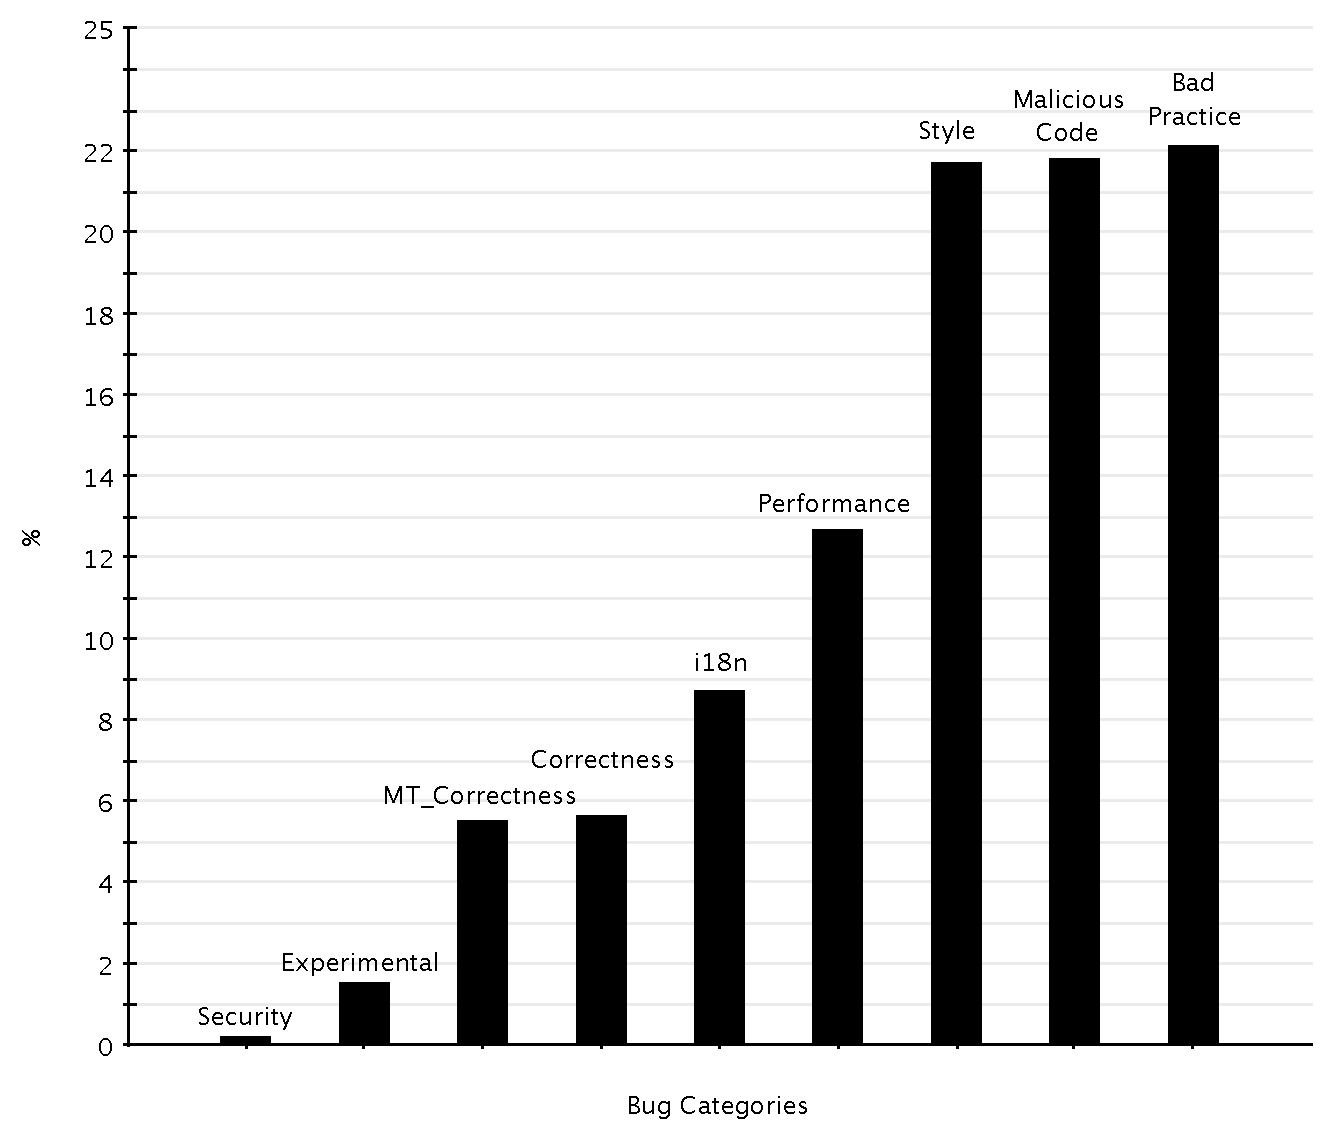
\includegraphics[scale=0.32]{figures/bug_percent}
	\caption{Bug percentage in Maven repository.}
	\label{fig:bug-per} 
\end{figure}

Since Mongo{\sc db} provides a rich query interface,
it was easy to either create
queries to find out basic information like:
``how many bad practice bugs exist in the repository", or
create scripts that can help us capture correlations
that could provide interesting findings. For instance,
Figure~\ref{fig:bug-per} shows how software 
bugs are distributed among the repository.

Together with our dataset, we have created a series of
scripts to exhibit how it can be used regarding
the evolution of software bugs.
Table~\ref{tbl:bugsperversion} shows the relation between
bugs and time. This relation, can be traced from the number of
bugs per category in each project version. We can then calculate the
Spearman correlations between the defects count and the ordinal
version number across all projects to see if bigger versions relate to
higher or lower defect counts.
The zero tendency though, applies to all versions of all projects together.
Thus, we also performed Spearman correlations between bug counts and version
ordinals in all projects we examined individually. These paint a different picture
from the above table, shown in Figure~\ref{fig:bugsversionscorr}. The
spike in point zero is explained by the large number of projects for
which no correlation could be established---the scale is
logarithmic.
Figure~\ref{fig:bugdiffs}, presents a histogram of the changes
of different bug counts in
project versions. In most cases, a bug count does not change between
versions; but when it does change, it may change upwards or downwards.

\begin{table}[tphp]
    \centering
    \caption{Correlations between version and defects count.}
    \label{tbl:bugsperversion}
    
\begin{tabular}{lcc}
\hline \\
Category & Spearman Correlation & $p$-value \\ \hline 
Security & 0.04 & $< 0.05$\\
Malicious Code & 0.03 & $\ll 0.05$\\
Style & 0.03 & $\ll 0.05$\\
Correctness & 0.04 & $\ll 0.05$\\
Bad Practice & 0.03 & $\ll 0.05$\\
{\sc mt} Correctness & 0.09 & $\ll 0.05$\\
i18n & 0.06 & $\ll 0.05$\\
Performance & {\it (0.01) } & 0.07\\
Experimental & 0.09 & $\ll 0.05$\\
\hline \\
\end{tabular}

\end{table}

\begin{figure*}[p]
  \centering
  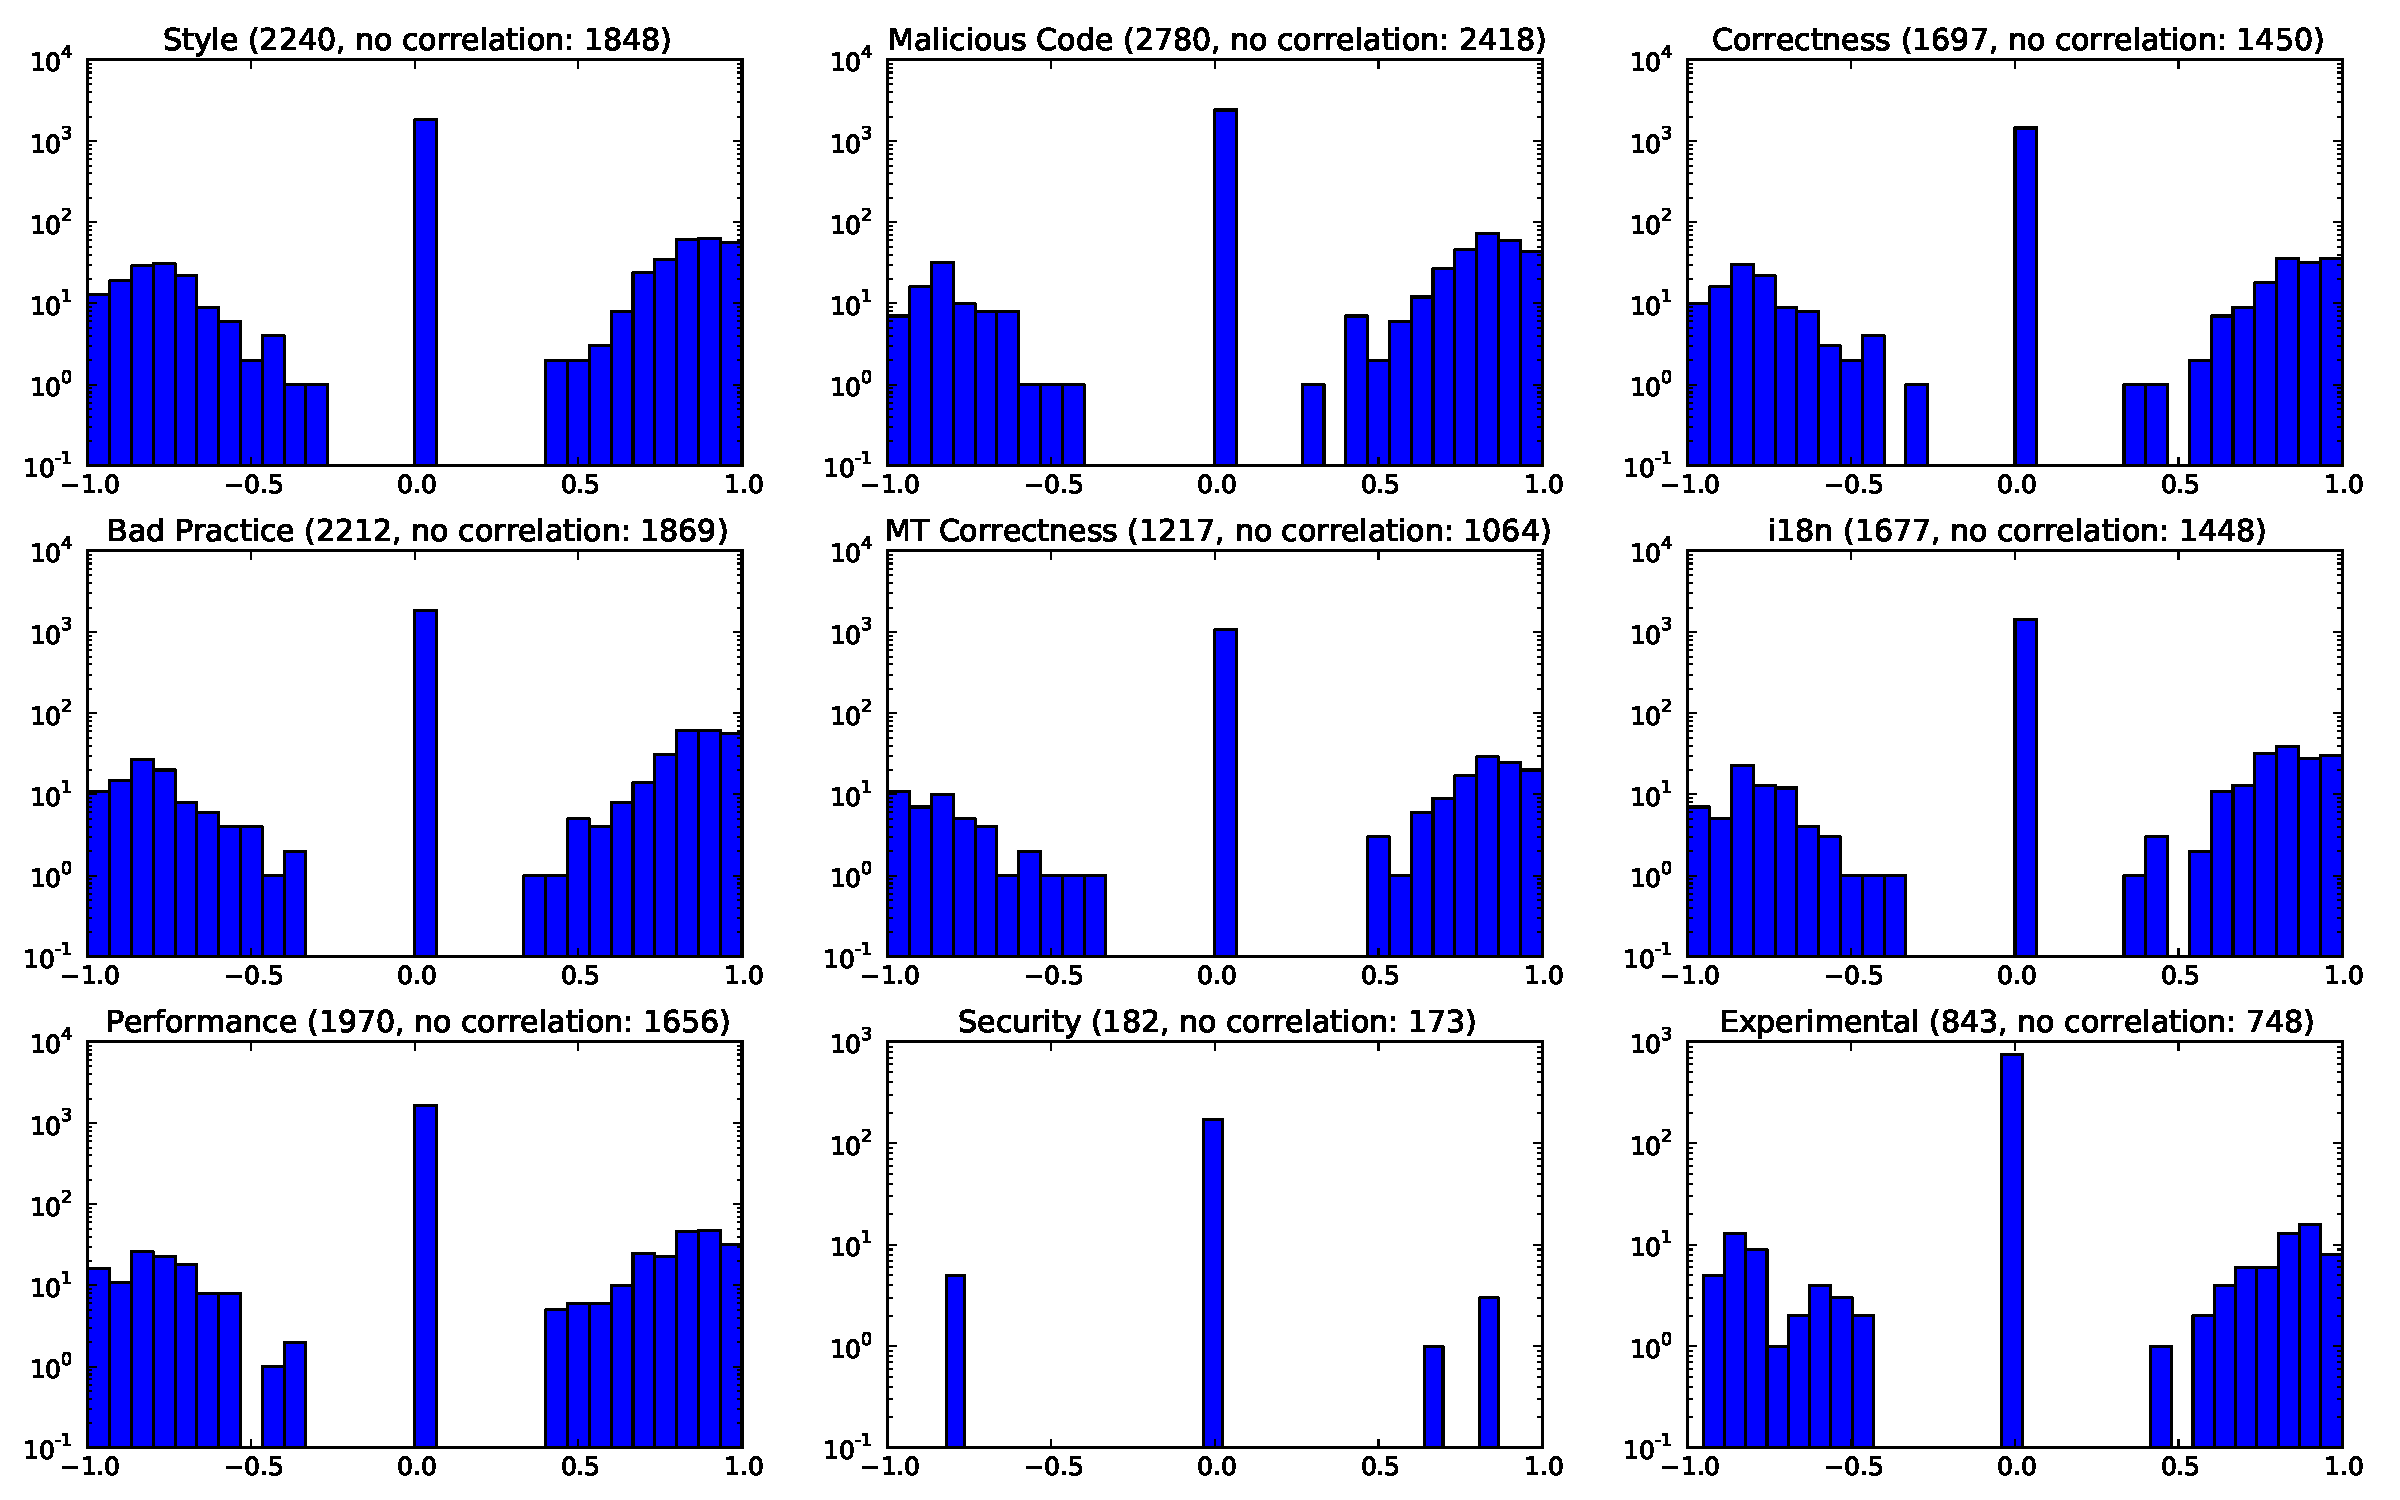
\includegraphics[scale=0.30]{bugsversionscorr}
  \caption{Histograms of correlations between bug counts and version
    ordinals per project. In brackets the total population size and
    the number of no correlation instances.}
  \label{fig:bugsversionscorr}
  \centering
  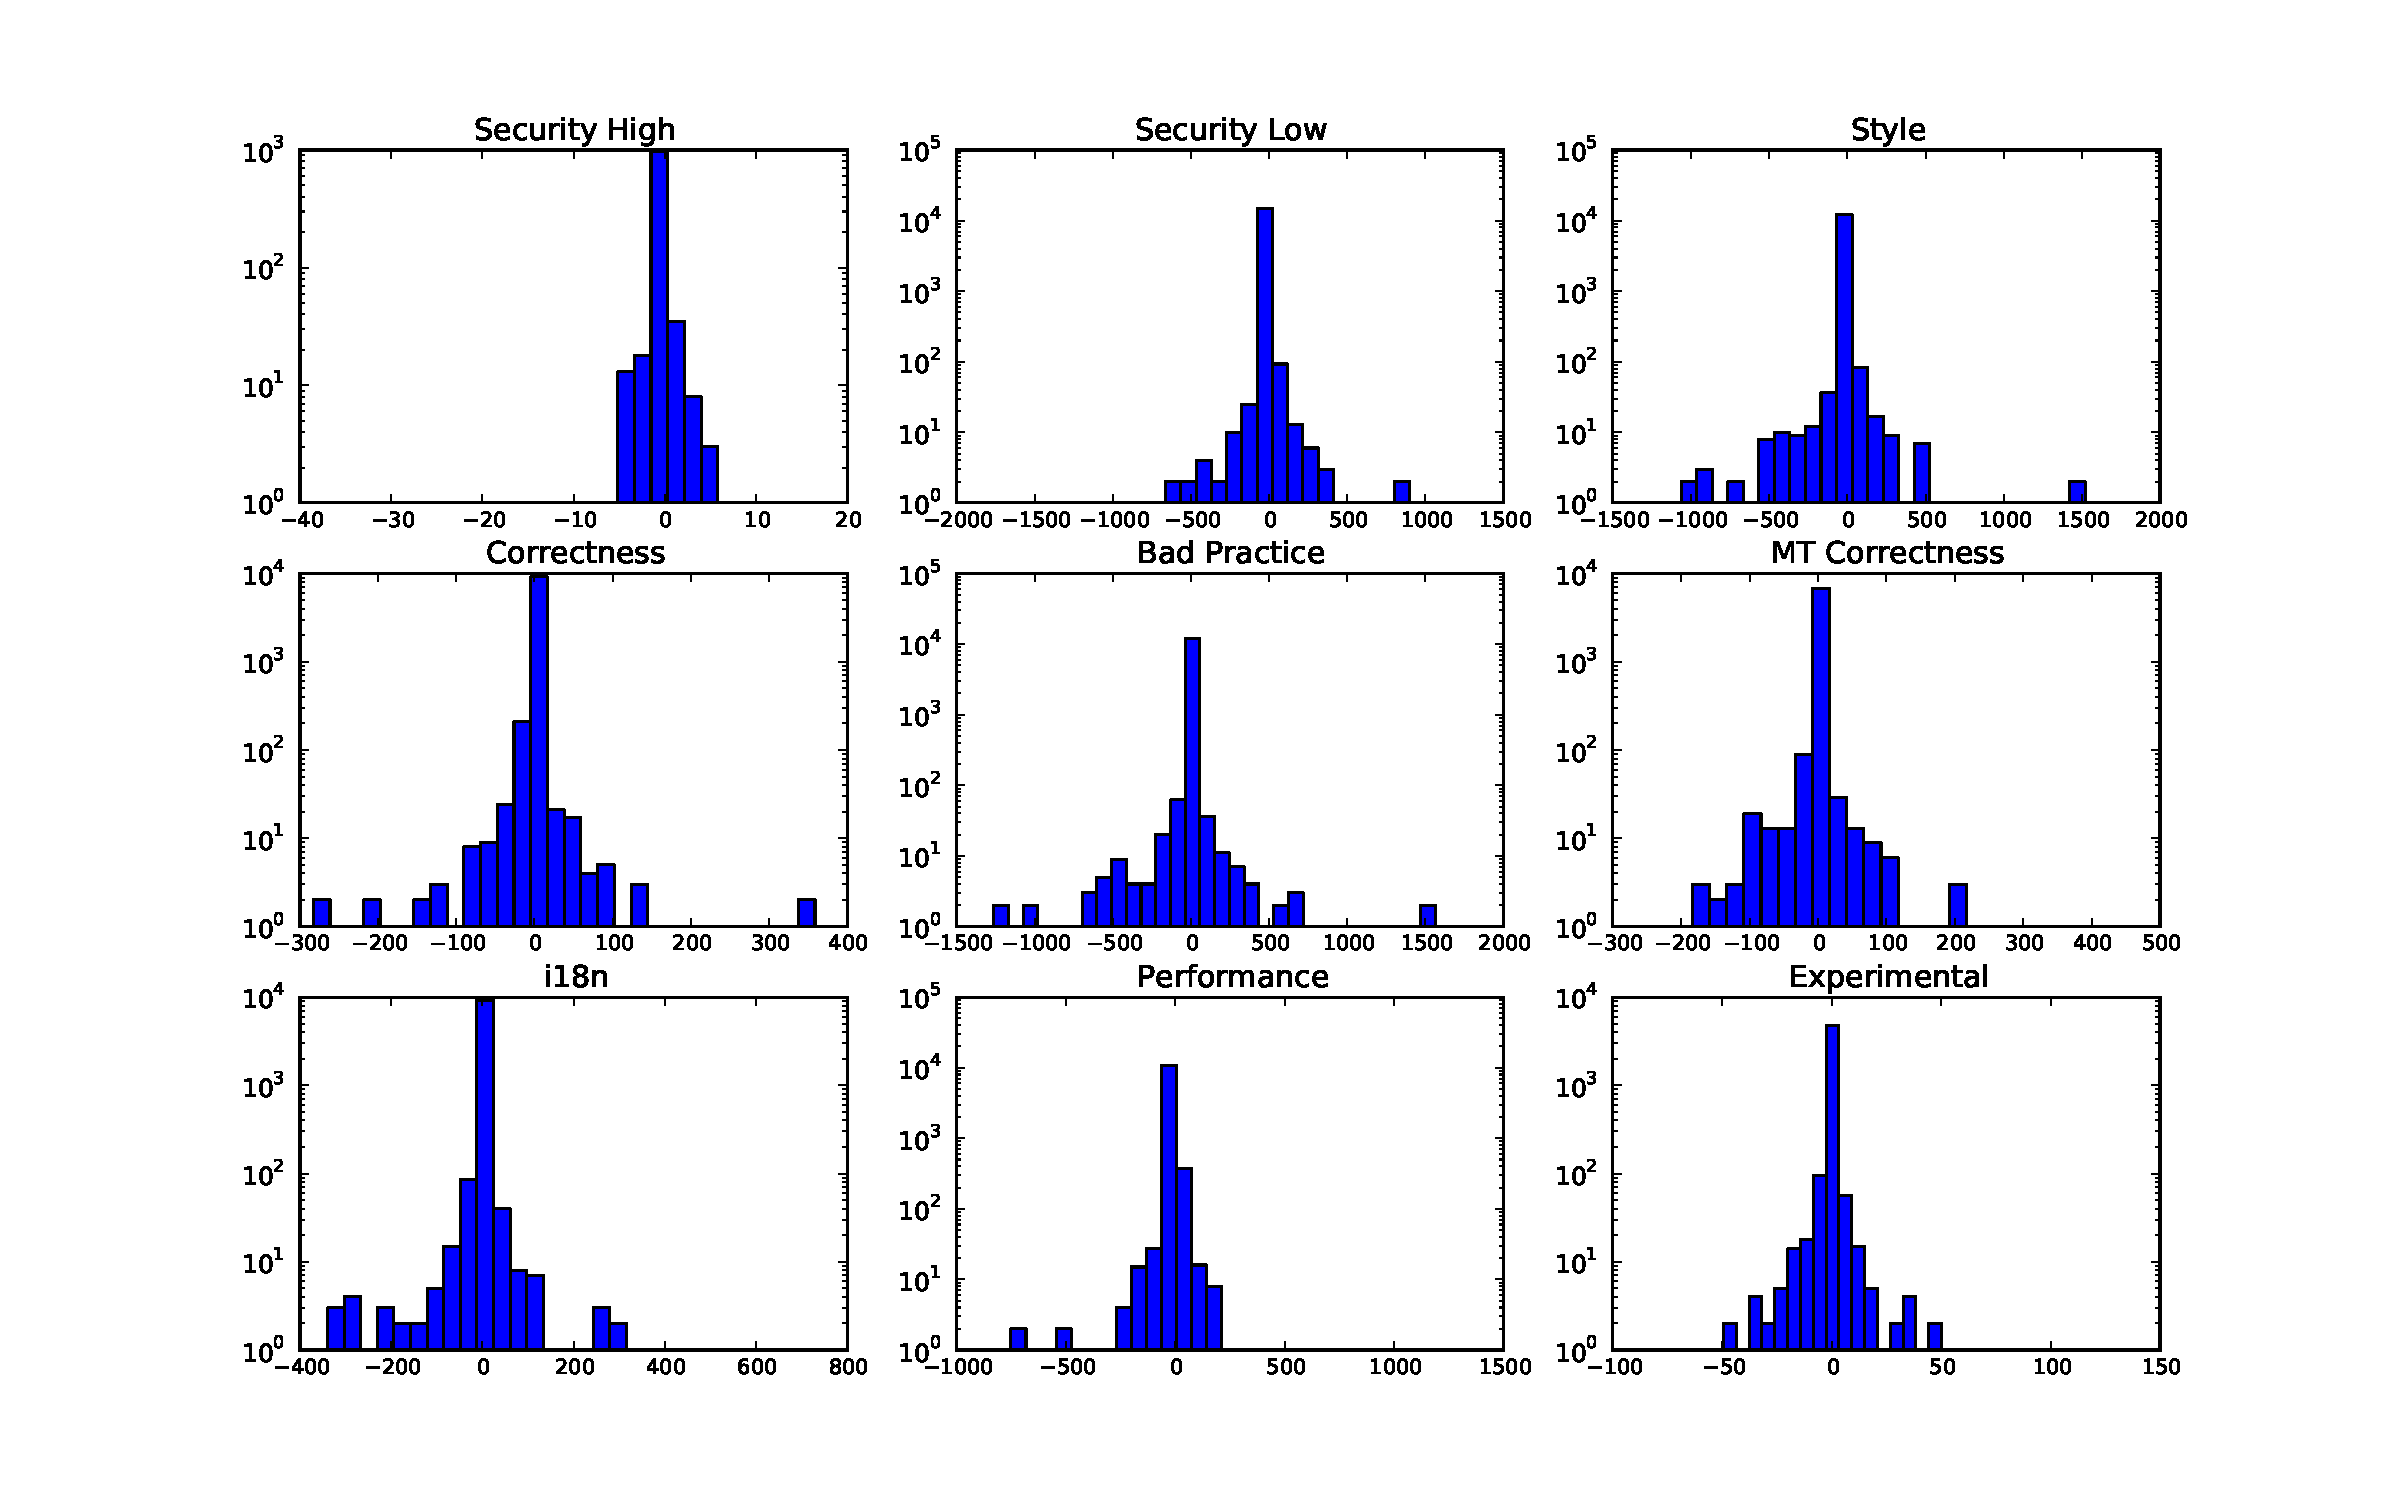
\includegraphics[scale=0.35]{bugdiffs}
  \caption{Changes in bug counts between versions.}
  \label{fig:bugdiffs}
\end{figure*}

To examine the relation between the persistence of different kinds of
bugs we used as a persistence
indicator the number of versions a bug remains open in a project. To
``tag" a bug we created a bug identifier by using the type of the bug,
the method name and the class name in which the bug was found in. We
chose not to use the line number of the location of the bug since it
could change from version to version and after a possible code
refactoring. We grouped the persistence numbers by bug categories and
then performed a Mann-Whitney $U$~\cite{HM98} test among all bug
category pairs. The results are presented in
Table~\ref{tbl:bug_persistence} (at the end of this paper). Cells in
brackets show pairs where no statistically significant difference was
found.

In addition, we explored the relation between defects with the size of a project
version, measured by the size of its {\sc jar} file by carrying out
correlation tests between the size and the defect counts for each
project and version. The results can be seen in
Table~\ref{tbl:jarsizecorr}.

Finally, Figure~\ref{fig:corrplot} presents the pairwise correlations
between all bug categories. To establish these correlations,
we calculated the
correlations between the number of distinct bugs that appeared in
a project throughout its lifetime.

\begin{table}[hbt]
    \centering
    \caption{Correlations between {\sc jar} size and defects count.}
    \label{tbl:jarsizecorr}
    
\begin{tabular}{lcc}
\hline \\
Category & Spearman Correlation & $p$-value \\ \hline 
Security & 0.19 & $\ll 0.05$\\
Malicious Code & 0.65 & $\ll 0.05$\\
Style & 0.68 & $\ll 0.05$\\
Correctness & 0.51 & $\ll 0.05$\\
Bad Practice & 0.67 & $\ll 0.05$\\
{\sc mt} Correctness & 0.51 & $\ll 0.05$\\
i18n & 0.53 & $\ll 0.05$\\
Performance & 0.63 & $\ll 0.05$\\
Experimental & 0.36 & $\ll 0.05$\\
\hline \\
\end{tabular}

\end{table}


\begin{figure}
  \centering
  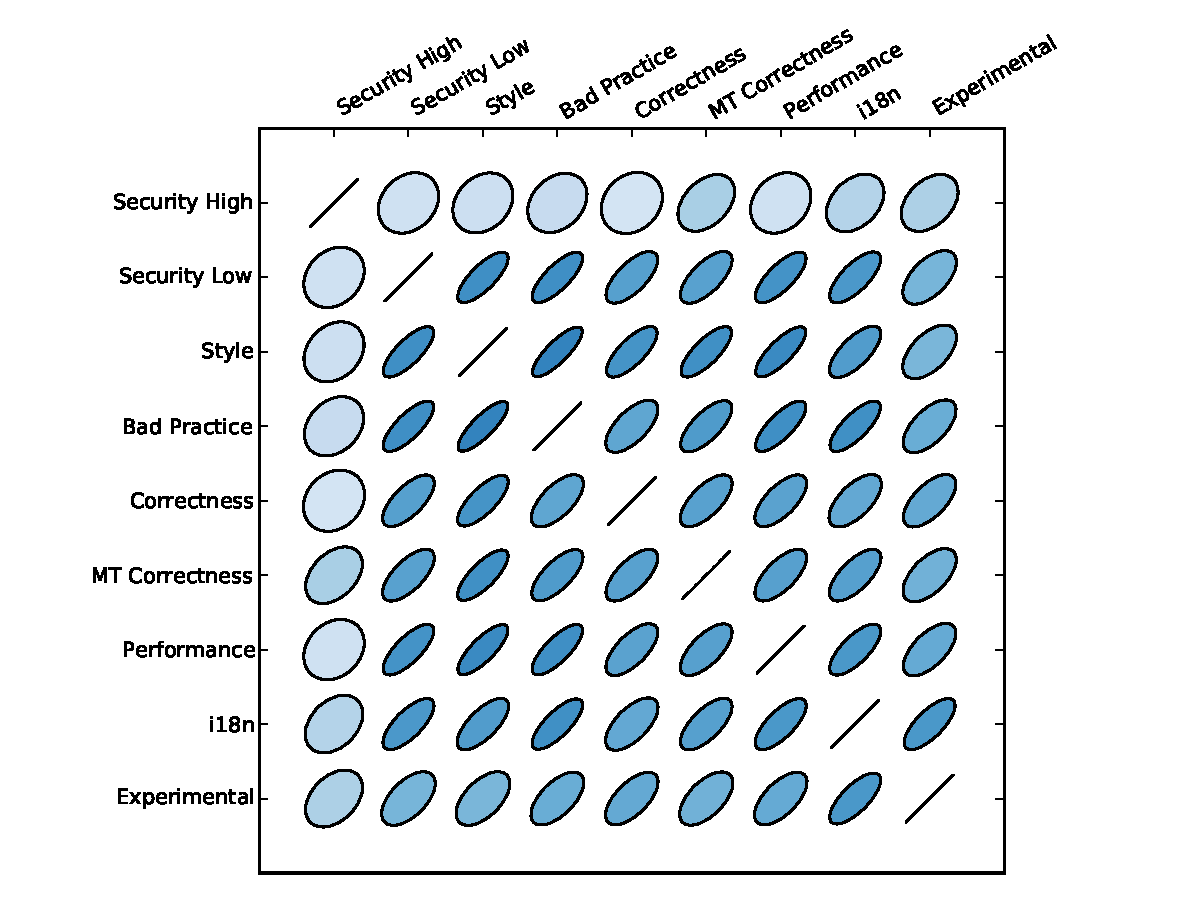
\includegraphics[scale=0.43]{corrplot.pdf}
  \caption{Correlation matrix plot for bug categories.}
  \label{fig:corrplot}
\end{figure}

\section{Related Work}
\label{sec:rel}

The Maven ecosystem has been previously analyzed by
Raemaekers et al.~\cite{RDV13}
to produce the {\it Maven dependency dataset}.
Apart from basic information like individual methods, classes,
packages and lines of code for every {\sc jar}, this dataset
also includes a database with all the
connections between the aforementioned elements.

\section{Conclusions}
\label{sec:conc}

In this paper, we have presented a dataset that contains
for every {\sc jar} of the Maven Central Repository,
all the software bug that it contains among with some
other metadata. We have also shown how our data can be
used to extract results concerning software evolution.
Research concerning the examination of specific bugs
can be facilitated by our dataset. For instance,
we have examined the characteristics of security
bugs in a previous paper, based upon this dataset~\cite{MKLGS13}.

The complete set of our data and source code
can be found at
\url{https://github.com/bkarak/data_paper_msr2014}.

\bibliographystyle{abbrv}
\bibliography{msr}  

\begin{landscape}
  \begin{table}
    \setlength{\extrarowheight}{0.10cm}
    \caption{Bug persistence comparison.}
    \label{tbl:bug_persistence}
    \resizebox{0.95\columnwidth}{!}{
    
\begin{tabular}{|l|>{\centering\arraybackslash}m{2.5cm}|>{\centering\arraybackslash}m{2.5cm}|>{\centering\arraybackslash}m{2.5cm}|>{\centering\arraybackslash}m{2.5cm}|>{\centering\arraybackslash}m{2.5cm}|>{\centering\arraybackslash}m{2.5cm}|>{\centering\arraybackslash}m{2.5cm}|>{\centering\arraybackslash}m{2.5cm}|}
\hline 
Security & {\it ($0.19$, $p = 0.85$\newline 2.86, 2.36\newline 265, 35026)} & $2.48$, $p < 0.05$\newline 2.86, 2.12\newline 265, 49043 & {\it ($-0.38$, $p = 0.70$\newline 2.86, 2.50\newline 265, 12905)} & $3.05$, $p < 0.01$\newline 2.86, 2.11\newline 265, 49324 & {\it ($1.22$, $p = 0.22$\newline 2.86, 2.48\newline 265, 10227)} & {\it ($-1.10$, $p = 0.27$\newline 2.86, 2.74\newline 265, 10718)} & {\it ($-0.90$, $p = 0.37$\newline 2.86, 2.65\newline 265, 23598)} & {\it ($-0.20$, $p = 0.84$\newline 2.86, 2.85\newline 265, 2686)}\\
Malicious Code &  & $20.25$, $p \ll 0.05$\newline 2.36, 2.12\newline 35026, 49043 & $-3.59$, $p \ll 0.05$\newline 2.36, 2.50\newline 35026, 12905 & $25.16$, $p \ll 0.05$\newline 2.36, 2.11\newline 35026, 49324 & $5.58$, $p \ll 0.05$\newline 2.36, 2.48\newline 35026, 10227 & $-7.55$, $p \ll 0.05$\newline 2.36, 2.74\newline 35026, 10718 & $-8.20$, $p \ll 0.05$\newline 2.36, 2.65\newline 35026, 23598 & {\it ($-1.39$, $p = 0.16$\newline 2.36, 2.85\newline 35026, 2686)}\\
Style &  &  & $-17.96$, $p \ll 0.05$\newline 2.12, 2.50\newline 49043, 12905 & $5.66$, $p \ll 0.05$\newline 2.12, 2.11\newline 49043, 49324 & $-6.84$, $p \ll 0.05$\newline 2.12, 2.48\newline 49043, 10227 & $-20.61$, $p \ll 0.05$\newline 2.12, 2.74\newline 49043, 10718 & $-26.18$, $p \ll 0.05$\newline 2.12, 2.65\newline 49043, 23598 & $-8.30$, $p \ll 0.05$\newline 2.12, 2.85\newline 49043, 2686\\
Correctness &  &  &  & $21.38$, $p \ll 0.05$\newline 2.50, 2.11\newline 12905, 49324 & $7.44$, $p \ll 0.05$\newline 2.50, 2.48\newline 12905, 10227 & $-3.57$, $p \ll 0.05$\newline 2.50, 2.74\newline 12905, 10718 & $-2.91$, $p < 0.01$\newline 2.50, 2.65\newline 12905, 23598 & {\it ($0.40$, $p = 0.69$\newline 2.50, 2.85\newline 12905, 2686)}\\
Bad Practice &  &  &  &  & $-10.02$, $p \ll 0.05$\newline 2.11, 2.48\newline 49324, 10227 & $-23.63$, $p \ll 0.05$\newline 2.11, 2.74\newline 49324, 10718 & $-30.32$, $p \ll 0.05$\newline 2.11, 2.65\newline 49324, 23598 & $-9.98$, $p \ll 0.05$\newline 2.11, 2.85\newline 49324, 2686\\
{\sc mt} Correctness &  &  &  &  &  & $-10.17$, $p \ll 0.05$\newline 2.48, 2.74\newline 10227, 10718 & $-10.83$, $p \ll 0.05$\newline 2.48, 2.65\newline 10227, 23598 & $-4.03$, $p \ll 0.05$\newline 2.48, 2.85\newline 10227, 2686\\
i18n &  &  &  &  &  &  & {\it ($1.29$, $p = 0.20$\newline 2.74, 2.65\newline 10718, 23598)} & $2.46$, $p < 0.05$\newline 2.74, 2.85\newline 10718, 2686\\
Performance &  &  &  &  &  &  &  & {\it ($1.92$, $p = 0.05$\newline 2.65, 2.85\newline 23598, 2686)}\\
\hline
\multicolumn{1}{l|}{}  &  &  &  &  &  &  &  &  \\
\cline{1-1}
\multicolumn{2}{l|}{Malicious Code}  &  &  &  &  &  &  &  \\
\cline{1-2}
\multicolumn{3}{l|}{Style}  &  &  &  &  &  &  \\
\cline{1-3}
\multicolumn{4}{l|}{Correctness}  &  &  &  &  &  \\
\cline{1-4}
\multicolumn{5}{l|}{Bad Practice}  &  &  &  &  \\
\cline{1-5}
\multicolumn{6}{l|}{MT Correctness}  &  &  &  \\
\cline{1-6}
\multicolumn{7}{l|}{i18n}  &  &  \\
\cline{1-7}
\multicolumn{8}{l|}{Performance}  &  \\
\cline{1-8}
\multicolumn{9}{l|}{Experimental}  \\
\cline{1-9}
\hline
\end{tabular}
}\\
    The matrix presents pairwise Mann-Whitney $U$ test results
    between the different bug categories. Each cell contains the test
    result (the value of $U$), the $p$-value, the average for each
    category and the sample size for each category. Cells in brackets show
    pairs where no statistically significant difference was found.
  \end{table}
\end{landscape}

\end{document}
